\documentclass{article}
\usepackage[utf8]{inputenc}
\usepackage{tikz}

\title{flow}
\author{Iwo Gross}
\date{December 2022}
\usetikzlibrary{shapes.geometric, arrows, animations}


\tikzstyle{output} = [diamond, aspect=2, text centered, draw=black,thick, minimum width=3cm, minimum height=1cm, text width=2cm]
\tikzstyle{data} = [rectangle, rounded corners, text centered, draw=black,thick, minimum width=2cm, minimum height=1cm]
\tikzstyle{input} = [ellipse, text centered, draw=black,thick, minimum width=3cm, minimum height=1cm, text width=2cm]
\tikzstyle{function} = [rectangle, text centered, draw=black,thick, fill=black!15, minimum width=3cm, minimum height=1cm]
\tikzstyle{arrow} = [thick, ->, >=stealth]

\begin{document}
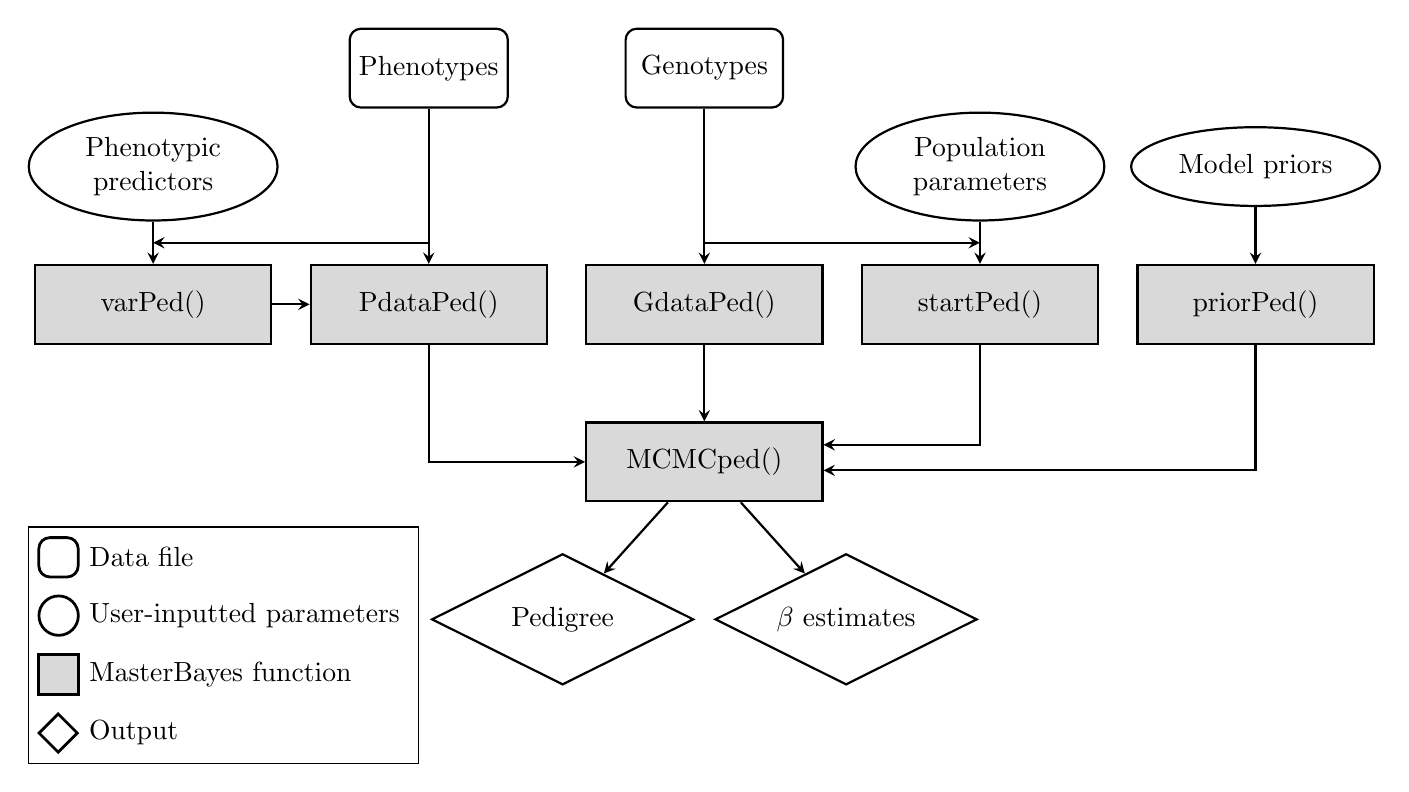
\begin{tikzpicture}[node distance=2cm,
datanode/.style={shape= rectangle, rounded corners, draw=black, minimum height = 0.5cm, minimum width=0.5cm, line width=1},
inputnode/.style={shape= ellipse, draw=black, minimum height = 0.5cm, minimum width=0.5cm, line width=1},
functionnode/.style={shape= rectangle, fill=black!15, draw=black, minimum height = 0.5cm, minimum width=0.5cm, line width=1},
outputnode/.style={shape= diamond, draw=black, minimum height = 0.5cm, minimum width=0.5cm, line width=1}
]


\node (finalped) [output] {Pedigree};
\node (finalbeta) [output, right of=finalped, xshift=1.6cm] {$\beta$ estimates};
\node (mcmcped) [function, above of = finalped, xshift=1.8cm] {MCMCped()};
\node (gdataped) [function, above of = mcmcped] {GdataPed()};
\node (pdataped) [function, left of = gdataped, xshift=-1.5cm] {PdataPed()};
\node (startped) [function, right of = gdataped, xshift=1.5cm] {startPed()};
\node (priorped) [function, right of = startped, xshift=1.5cm] {priorPed()};
\node (priors) [input, above of = priorped, yshift=-.25cm] {Model priors};
\node (guppyg) [data, above of = gdataped, yshift=1cm] {Genotypes};
\node (varped) [function, left of = pdataped, xshift=-1.5cm] {varPed()};
\node (preds) [input, above of = varped, yshift=-.25cm] {Phenotypic predictors};
\node (guppyp) [data, above of = pdataped, yshift=1cm] {Phenotypes};
\node (params) [input, above of = startped, yshift=-.25cm] {Population parameters};

\draw [arrow] (mcmcped) -- (finalped);
\draw [arrow] (mcmcped) -- (finalbeta);
\draw [arrow] (gdataped) -- (mcmcped);
\draw [arrow] (pdataped) |- (mcmcped);
\draw [arrow] (startped) |- ([yshift=0.5cm]mcmcped);
\draw [arrow] (priorped) |- ([yshift=-0.5cm]mcmcped);
\draw [arrow] (guppyg) -- (gdataped);
\draw [arrow] (varped) -- (pdataped);
\draw [arrow] (preds) --coordinate[midway](m1) (varped);
\draw [arrow] (guppyp) -- (pdataped);
\draw [arrow] (guppyp) |- (m1);
\draw [arrow] (params) --coordinate[midway](m2)(startped);
\draw [arrow] (guppyg) |- (m2);
\draw [arrow] (priors) -- (priorped);

\matrix [draw,above right, row sep=2mm, yshift=-1cm] at (current bounding box.south west) {
  \node [datanode,label=right:Data file]{}; \\
  \node [inputnode,label=right:User-inputted parameters, xshift=.08cm]{}; \\
  \node [functionnode,label=right:MasterBayes function,]{}; \\
  \node [outputnode,label=right:Output, xshift=.13cm]{}; \\
};
\end{tikzpicture}
\end{document}
